\begin{figure}[!h]

\begin{center}
\resizebox{\textwidth}{!}{%
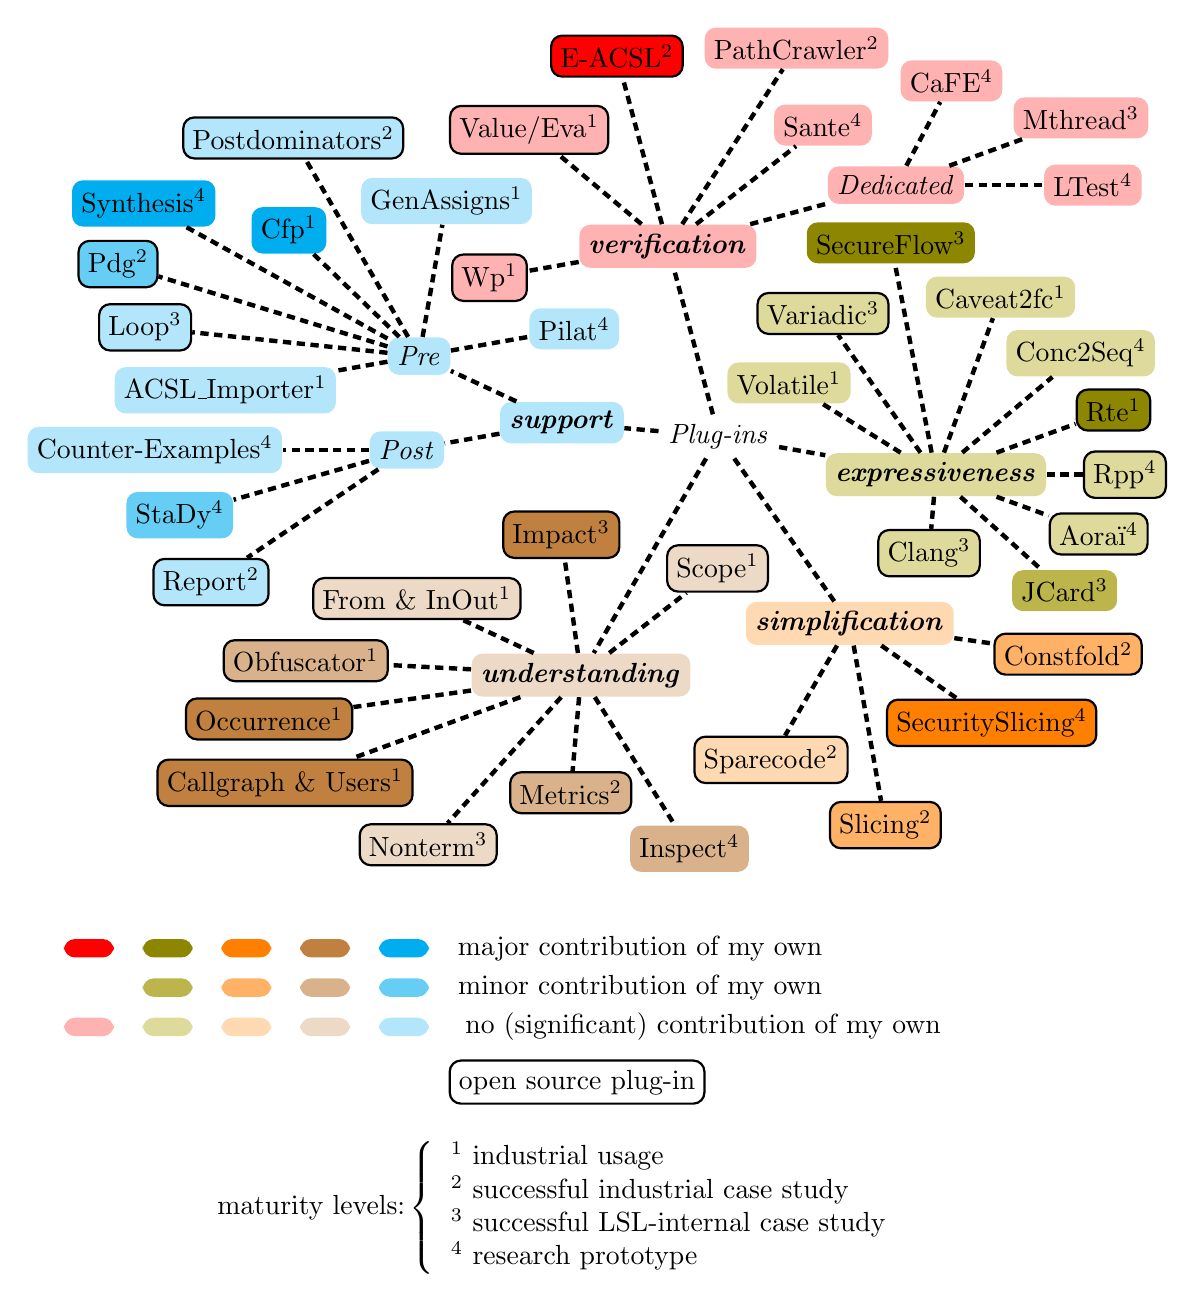
\begin{tikzpicture}[
  x=1mm,y=1mm,
  edge from parent path={[draw,ultra thick, densely dashed]
      (\tikzparentnode\tikzparentanchor) -- (\tikzchildnode\tikzchildanchor)},
  concept/.style={rectangle, rounded corners, minimum height=0mm},
  opensource/.style={draw=black, thick, solid}
  ]
%
\node[concept] {\textit{Plug-ins}}
%
% verification
child[grow=105 clockwise, concept/.append, level distance=25mm]
{node[concept,fill=red!30] { \textbf{\textit{verification }}}
  %% child[grow=210 clockwise, concept/.append, level distance=18mm]
  %% { node[concept,fill=red!30] { Jessie } }
  child[grow=190 clockwise, concept/.append, level distance=23mm]
  { node[concept,fill=red!30,opensource] { Wp$^1$ } }
  child[grow=140 clockwise, concept/.append, level distance=23mm]
  { node[concept,fill=red!30,opensource] { Value/Eva$^1$ } }
  child[grow=105 clockwise, concept/.append, level distance=25mm]
  { node[concept,fill=red,opensource] { E-ACSL$^2$ }}
  child[grow=57 clockwise, concept/.append, level distance=30mm]
  { node[concept,fill=red!30] { PathCrawler$^2$ } }
  child[grow=38 clockwise, concept/.append, level distance=25mm]
  { node[concept,fill=red!30] { Sante$^4$ } }
  child[grow=15 clockwise, concept/.append, level distance=30mm]
  { node[concept,fill=red!30] { \textit{Dedicated} }
    child[grow=62 clockwise, concept/.append, level distance=15mm]
    { node[concept,fill=red!30] { Ca{FE}$^4$ } }
    child[grow=20 clockwise, concept/.append, level distance=25mm]
    { node[concept,fill=red!30] { Mthread$^3$ } }
    child[grow=0 clockwise, concept/.append, level distance=25mm]
    { node[concept,fill=red!30] { LTest$^4$ } }
  }
}
%
% expressiveness
child[grow=-10 clockwise, concept/.append, level distance=28mm]
{node[concept,fill=olive!30] { \textbf{\textit{expressiveness}} }
  child[grow=-95 clockwise, concept/.append, level distance=10mm]
  { node[concept,opensource,fill=olive!30] { Clang$^3$ } }
  child[grow=-42 clockwise, concept/.append, level distance=22mm]
  { node[concept,fill=olive!60] { JCard$^3$ } }
  child[grow=-20 clockwise, concept/.append, level distance=22mm]
  { node[concept,opensource,fill=olive!30] { Aora\"i$^4$ } }
  child[grow=0 clockwise, concept/.append, level distance=24mm]
  { node[concept,opensource,fill=olive!30] { Rpp$^4$ } }
  child[grow=20 clockwise, concept/.append, level distance=24mm]
  { node[concept,opensource,fill=olive] { Rte$^1$ } }
  child[grow=40 clockwise, concept/.append, level distance=24mm]
  { node[concept,fill=olive!30] { Conc2Seq$^4$ } }
  child[grow=70 clockwise, concept/.append, level distance=24mm]
  { node[concept,fill=olive!30] { Caveat2fc$^1$ } }
  child[grow=101 clockwise, concept/.append, level distance=30mm]
  { node[concept,fill=olive] { SecureFlow$^3$ } }
  child[grow=125 clockwise, concept/.append, level distance=25mm]
  { node[concept,opensource, fill=olive!30] { Variadic$^3$ } }
  child[grow=148 clockwise, concept/.append, level distance=22mm]
  { node[concept,fill=olive!30] { Volatile$^1$ } }
}
%
% simplification
child[grow=-55 clockwise, concept/.append, level distance=29mm]
{node[concept,fill=orange!30] { \textbf{\textit{simplification}} }
  child[grow=-8 clockwise, concept/.append, level distance=28mm]
  { node[concept,opensource,fill=orange!60] { Constfold$^2$ } }
  child[grow=-35 clockwise,concept/.append, level distance=22mm]
  { node[concept,opensource,fill=orange] { SecuritySlicing$^4$ } }
  child[grow=-80 clockwise,concept/.append, level distance=26mm]
  { node[concept,opensource, fill=orange!60] { Slicing$^2$ } }
  child[grow=-120 clockwise, concept/.append, level distance=20mm]
  { node[concept,opensource,fill=orange!30] { Sparecode$^2$ } }
}
%
% understanding
child[grow=-120 clockwise, concept/.append, level distance=35mm]
{node[concept,fill=brown!30] { \textbf{\textit{understanding}} }
  child[grow=-58 clockwise, concept/.append, level distance=26mm]
  { node[concept,fill=brown!60] { Inspect$^4$ } }
  child[grow=-95 clockwise, concept/.append, level distance=15mm]
  { node[concept,opensource,fill=brown!60] { Metrics$^2$ } }
  child[grow=-132 clockwise, concept/.append, level distance=29mm]
  { node[concept,opensource,fill=brown!30] { Nonterm$^3$ } }
  child[grow=-160 clockwise, concept/.append, level distance=40mm]
  { node[concept,opensource,fill=brown] { Callgraph \& Users$^1$ } }
  child[grow=-172 clockwise, concept/.append, level distance=40mm]
  { node[concept,opensource,fill=brown] { Occurrence$^1$ } }
  child[grow=-183 clockwise, concept/.append, level distance=35mm]
  { node[concept,opensource,fill=brown!60] { Obfuscator$^1$ } }
  child[grow=-205 clockwise,concept/.append, level distance=23mm]
  { node[concept, opensource,fill=brown!30] { From \& InOut$^1$ } }
  child[grow=-262 clockwise, concept/.append, level distance=18mm]
  { node[concept,opensource,fill=brown] { Impact$^3$ } }
  child[grow=38 clockwise, concept/.append, level distance=22mm]
  { node[concept,opensource,fill=brown!30] { Scope$^1$ } }
}
%
% support
child[grow=175 clockwise, concept/.append, level distance=20mm]
{node[concept,fill=cyan!30] { \textbf{\textit{support}} }
  child[grow=155 clockwise, concept/.append, level distance=20mm]
  { node[concept,fill=cyan!30] { \textit{Pre}}
    child[grow=10 clockwise, concept/.append, level distance=20mm]
    { node[concept,fill=cyan!30] { Pilat$^4$ } }
    child[grow=80 clockwise, concept/.append, level distance=20mm]
    { node[concept,fill=cyan!30] { GenAssigns$^1$ } }
    child[grow=120 clockwise, concept/.append, level distance=32mm]
    { node[concept,opensource,fill=cyan!30] { Postdominators$^2$ } }
    child[grow=136 clockwise, concept/.append, level distance=23mm]
    { node[concept,fill=cyan] { Cfp$^1$ } }
    child[grow=151 clockwise, concept/.append, level distance=40mm]
    { node[concept,fill=cyan] { Synthesis$^4$ } }
    child[grow=163 clockwise, concept/.append, level distance=40mm]
    { node[concept,opensource,fill=cyan!60] { Pdg$^2$ } }
    child[grow=174 clockwise,concept/.append, level distance=35mm]
    { node[concept, opensource,fill=cyan!30] { Loop$^3$ } }
    child[grow=190 clockwise, concept/.append, level distance=25mm]
    { node[concept,fill=cyan!30] { ACSL\_Importer$^1$ } }
  }
  child[grow=190 clockwise, concept/.append, level distance=20mm]
  { node[concept,fill=cyan!30] { \textit{Post}}
    child[grow=180 clockwise, concept/.append, level distance=32mm]
    { node[concept,fill=cyan!30] { Counter-Examples$^4$ } }
    child[grow=196 clockwise, concept/.append, level distance=30mm]
    { node[concept,fill=cyan!60] { StaDy$^4$ } }
    child[grow=214 clockwise, concept/.append, level distance=30mm]
    { node[concept,opensource,fill=cyan!30] { Report$^2$ } }
  }
}
;
%
% My contributions
\node[concept, fill=red, minimum width=18,minimum height=3,] at (-80,-65) {};
\node[concept, fill=olive, minimum width=18,minimum height=3] at (-70,-65) {};
\node[concept, fill=orange, minimum width=18,minimum height=3,] at (-60,-65) {};
\node[concept, fill=brown, minimum width=18,minimum height=3,] at (-50,-65) {};
\node[concept, fill=cyan, minimum width=18,minimum height=3,] at (-40,-65) {};
\node[concept, minimum width=18,minimum height=3,] at (-10,-65) {major
  contribution of my own};

\node[concept, fill=olive!60, minimum width=18,minimum height=3] at (-70,-70)
     {};
\node[concept, fill=orange!60, minimum width=18,minimum height=3,] at (-60,-70)
     {};
\node[concept, fill=brown!60, minimum width=18,minimum height=3,] at (-50,-70)
     {};
\node[concept, fill=cyan!60, minimum width=18,minimum height=3,] at (-40,-70)
     {}; 
\node[concept, minimum width=18,minimum height=3,] at (-10,-70) {minor
  contribution of my own};

\node[concept, fill=red!30, minimum width=18,minimum height=3,] at (-80,-75) {};
\node[concept, fill=olive!30, minimum width=18,minimum height=3] at (-70,-75)
     {};
\node[concept, fill=orange!30, minimum width=18,minimum height=3,] at (-60,-75)
     {};
\node[concept, fill=brown!30, minimum width=18,minimum height=3,] at (-50,-75)
     {};
\node[concept, fill=cyan!30, minimum width=18,minimum height=3,] at (-40,-75)
     {}; 
\node[concept, minimum width=18,minimum height=3,] at (-2,-75) {no
  (significant) contribution of my own};

%
% Open Source
\node[concept, opensource, minimum width=18,minimum height=3,] at (-18,-82)
     {open source plug-in};
%
% Maturity level
\node at  (-20,-98) {%
  $\mbox{maturity levels:}
  \left\{
  \begin{tabular}{l}
    $^1$ industrial usage \\
    $^2$ successful industrial case study \\
    $^3$ successful LSL-internal case study \\
    $^4$ research prototype
  \end{tabular}\right.$};

\end{tikzpicture}
} % resizebox
\end{center}

\caption{Greffons open-source du CEA}\label{fig:gallery}
%\caption{LSL's \framac Plug-in Gallery.}\label{fig:gallery}
\end{figure}

